\section{Durchführung}

    In diesem Versuch werden Fehlstellen in einem Plexiglasquader lokalisiert,
    sowie die Abstände in einem Augemodell gemessen.\\
    \\
    Für die Messung stehen ein Ultraschallechoskop,
    eine Ultraschallsonde mit einer Frequenz von $\SI{2}{\mega\hertz}$ und ein Computer mit einem Messprogramm zur Verfügung.
    Das Programm verfügt über die Einstellung der Laufzeit- und Tiefenmessung,
    wobei in diesem Versuch die Laufzeiten der Schallimpulse und die zugehörigen Spannungsamplituden gemessen werden. 
    Mit einem Curser können die Piks der Spannung,
    welche bei Fehlstellen in der Probe entstehen,
    genau gemessen werden,
    wobei hier das Impuls-Echo-Verfahren verwendet wird,
    welches in Abbildung \ref{fig:impuls_echo} in Kapitel \ref{sec:theorie} dargestellt ist.
    Es wird ein A-Scan durchgeführt.
    Als Kontaktmittel dienen bidestilliertes Wasser und Ultraschallgel,
    welches vor der Messung auf die Probe gegeben wird.
    Es muss darauf geachtet werden,
    dass die Sonde nicht zu stark auf die Probe gedrückt wird.

\subsection{Messung eines Acrylblocks mit Fehlstellen}

%Abbildung des Acrylblocks

    Zu Beginn wird der Acrylblock mithilfe einer Schieblehre ausgemessen,
    wobei diese Werte als Vergleich zur Ultraschallmessung dienen.
    Es werden die Seitenlängen,
    sowie die Abstände der Fehlstellen in dem Block von den Seiten gemessen.\\
    Anschließend wird destilliertes Wasser als Kontaktmittel auf eine Längs-Seite der Probe gegeben.
    Mit der Ultraschallsonde werden dann die Fehlstellen abgetastet,
    wobei die Laufzeit der Schallimpulse und die zugehörige Spannungsamplitude notiert werden.
    Bei einer vorher eingestellen Schallgeschwindigkeit von $c = \SI{2730}{\meter\per\second}$ können die Positionen der Fehlstellen mithilfe der Gleichung \eqref{eqn:position_fehlstelle} berechnet werden.\\
    Dann wird die Messung für die gegenüberliegende Seite des Acrlyblocks wiederholt.

\subsection{Messung der Abstände in einem Augenmodell}

    Für diesen Versuch steht ein Modell eines Auges zur Verfügung,
    welches in der folgenden Abbildung \ref{fig:augenmodell} vereinfacht dargestellt ist.

    \begin{figure}[H]
        \centering
        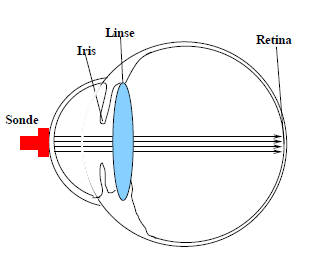
\includegraphics[scale=0.7]{augenmodell.PNG}
        \caption{Der schematische Aufbau des Auges.}
        \label{fig:augenmodell}
    \end{figure}

    Für die Messung mit der Ultraschallsonde wird Ultraschallgel verwendet,
    damit die Sonde leichter auf der Oberfläche des Auges bewegt werden kann.
    Es werden drei Piks gemessen,
    die von der Iris, der Linse und der Retina verursacht werden,
    und die entsprechenden Laufzeiten und Amplituden der Schallimpulse notiert.\\
    \\
    Nach Abschluss der Messungen müssen die Ultraschallsonde und die Proben mithilfe von weichen Tüchern und Wasser vorsichtig gereinigt werden.